\documentclass[aps,prl,floatfix,preprintnumbers,twocolumn,groupedaddress,nofootinbib]{revtex4-1}
\usepackage{amsmath,amsthm,amssymb,color,psfrag,url,latexsym,graphicx,epstopdf,slashed,xspace,hyperref,enumitem}
\hyphenpenalty=500
\usepackage{lineno}

\definecolor{darkred}{rgb}{0.6,0.0,0.0}
\definecolor{darkblue}{rgb}{0.0,0.0,0.5}
\definecolor{darkgreen}{rgb}{0.0,0.5,0.0}
\definecolor{brown}{rgb}{0.0,0.0,0.0}
\newcommand{\red}{\color{darkred}}
\newcommand{\blue}{\color{darkblue}}
\newcommand{\green}{\color{darkgreen}}

\newcommand{\rap}{y}
\newcommand{\be}{\begin{equation}}
\newcommand{\ee}{\end{equation}}
\newcommand{\bea}{\begin{eqnarray}}
\newcommand{\eea}{\end{eqnarray}}

\begin{document}
\preprint{MIT-CTP 4952}
\title{Telescoping Jet Substructure}

\author{Yang-Ting Chien$^{a,d}$}
\email{ytchien@mit.edu\\}

\author{Alex Emerman$^{c,d,e}$}
%\email{alex.emerman@gmail.com}

\author{Shih-Chieh Hsu$^b$}
%\email{schsu@uw.edu}

\author{Samuel Meehan$^b$}
%\email{smeehan12@gmail.com}

\author{Zachary Montague$^{a,b}$}
%\email{zacander.mon@gmail.com}

\affiliation{
$^a$ Center for Theoretical Physics, Massachusetts Institute of Technology, Cambridge, MA 02139\\
$^b$ Department of Physics, University of Washington, Seattle, WA 98195\\
$^c$ Department of Physics, Columbia University, New York, NY 10027\\
$^d$ Theoretical Division, T-2, Los Alamos National Laboratory, Los Alamos, NM 87545\\
$^e$ Physics Department, Reed College, Portland, OR 97202
}

\date{\today}
\linenumbers

\begin{abstract}
Jet substructure observables probe specific regions of Standard Model dynamics. We introduce a novel jet substructure calculus by exploiting the variation of observables with respect to varied phase-space boundaries quantified by the variability. We demonstrate this general method in boosted $W$ and top tagging using telescoping jet grooming and telescoping subjets and show it disentangles the information from subjet topology and subjet substructure. We find the excellent performance of the variability and its robustness against finite detector resolution. The variability enables us to utilize the isolation of a highly boosted $W$ caused by its colorlessness, a dominant feature over its two-prong structure. Our method provides a new direction in heavy particle tagging and paves the road toward complete and systematic jet studies using telescoping deconstruction.
\end{abstract}
\maketitle

As Run 2 of the Large Hadron Collider (LHC) accumulates more data, we probe the physics above the electroweak scale where massive Standard Model particles can carry energy much larger than their invariant masses. The hadronic decays of such boosted heavy particles result in jets of collimated particles with prong-like substructures. Many jet substructure variables have been designed and combined in a multivariate analysis to help tag these particles and increase discovery significances of beyond the Standard Model physics \cite{Abdesselam:2010pt,Altheimer:2012mn,Altheimer:2013yza,Adams:2015hiv,Larkoski:2017jix}. However, as many of these variables are correlated, getting more information out of a jet can be a challenging task. %deciphering the correlations among arbitrary sets of variables can be a challenging task.

Every jet substructure observable and grooming procedure has parameters which define the specific phase space the variable probes. The parameters include the very basic choice of the jet algorithm \cite{Ellis:1993tq,Catani:1993hr,Cacciari:2008gp,Dokshitzer:1997in,Wobisch:1998wt} and the jet radius $R$. Jet grooming parameters, for example, $z_{\rm cut}$ and $D_{\rm cut}$ in jet pruning \cite{Ellis:2009su,Ellis:2009me}, define the softness and noncollinearity of a discarded particle. %The parameter $\beta$ in $N$-subjettiness \cite{Thaler:2010tr} defines the weights on the angles from the axes to a particle, and the integer $N$ is also a discrete parameter.
Conventionally, one makes a single, optimal choice of parameters in an analysis which can neglect the full information the entire observable class contains.

Recently, Q-jets \cite{Ellis:2012sn} introduced non-determinism in jet clustering. The procedure probes each jet multiple times and quantifies differences among pruned jets using the mass volatility. It was then realized in telescoping jets \cite{Chien:2013kca} that by probing around dominant energy flow with multiple angular resolutions $\{R_i\}$, one can extract the full information contained in jets at all angular scales \cite{Chien:2014hla}. In this Letter we apply telescoping jets to analyze arbitrary jet observables and grooming procedures. We demonstrate the method in boosted hadronic $W$ and top tagging. The mass volatility is promoted to the variability of each observable with varying parameters.

In hadronic boosted two-body resonance decays, the resonance mass $M$ introduces a two-prong structure in the jet and an angular scale $\Theta\approx 2M/p_T$ between the two prongs, where $p_T$ is the transverse momentum of the heavy particle. On the other hand, the QCD background of quark and gluon jets has a falling mass distribution. However, near $M\pm\Delta m$ the background jets are also two-prong-like but fuzzier when $\Delta m\gg\Gamma$ where $\Gamma$ is the natural width of the resonance. Besides this nontrivial {\sl subjet topology}, the strong interaction dictates the formation of subjets with {\sl subjet substructures} and {\sl subjet superstructures} \cite{Gallicchio:2010sw} which are sensitive to the partonic origins of subjets. %We classify jet substructures into these three categories using subjets.

The above physics picture describes the situation in $W$ tagging. For top tagging, the top mass $M_t$ and the $W$ mass $M_W$ are not hierarchically separated therefore $\Theta_t \approx 2M_t/p_T^t$ and $\Theta_W \approx 2M_W/p_T^W$ can be comparable. This results in the generic three-prong structure in the hadronic top decay $t\rightarrow W+b \rightarrow q_1 + q_2 +b$. Near $M_t\pm \Delta m$ the selected background jets are again two-prong-like. Observables which distinguish three-prong jets from two-prong jets will help discriminate the background.

Given an arbitrary jet observable $\cal O$ with a parameter $a$,
the variation of the observable with respect to the sampling of parameters $\{a_i\}$ within $(a_{\rm min},a_{\rm max})$, or the {\sl variability}, is quantified by the coefficient of variation $v_{\cal O}^a$ defined as the ratio of the standard deviation and the mean of $\{{\cal O}_{a_i}\}$,
\be
    v_{\cal O}^a = \frac{\sigma({\cal O}_{a_i})}{\langle {\cal O}_{a_i}\rangle}\;.
\ee
Variations with respect to multiple varied parameters can be studied using the variability matrix. Much like the first derivative in calculus, the variability $v_{\cal O}^a$ measures the change of the observable $\cal O$ with respect to the change of the phase space boundary set by the parameter $a$. Instead of combining observables with different parameters in a multivariate analysis, the variability can give a trend of the observable variation.

\begin{figure*}
    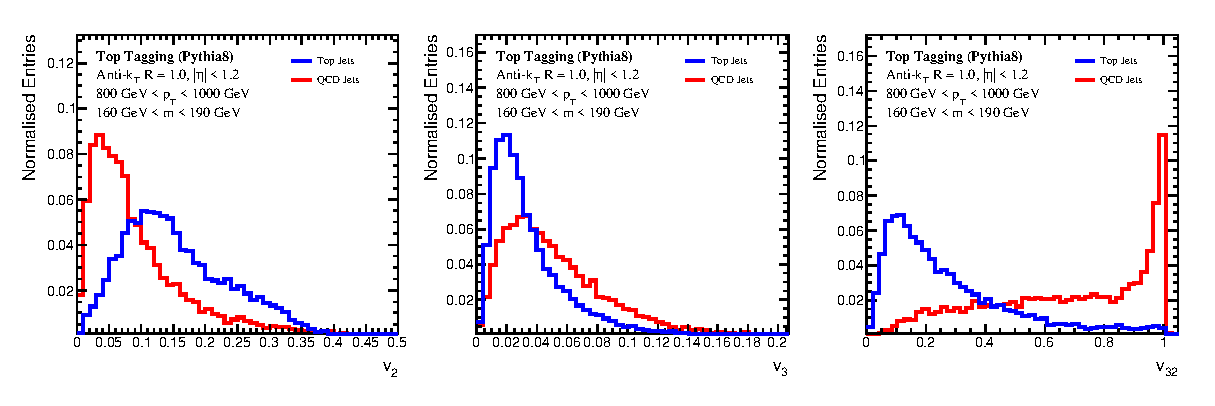
\includegraphics[width=2\columnwidth]{plots/Top_vs_high.eps}
    \caption{The distributions of the variabilities $v_2$ (left panel) and $v_3$ (middle panel), as well as their ratio $v_{32}$ (right panel) for top and QCD jets with $800~{\rm GeV} < p_T < 1~{\rm TeV}$ and $160~{\rm GeV} < m < 190~{\rm GeV}$ using the truth particle information.}
\label{v32}
\end{figure*}

We consider a variety of telescoping applications. We focus on the variability of the jet mass with respect to varying the parameters which determine the jet constituents contributing to the jet mass. %observable. In the construction of the variability variables, t
The sampling of the telescoping parameters is uniform within the range $(a_{\rm min},a_{\rm max})$. %\\[-10pt]

\noindent {\sl Telescoping pruning}: Using the $k_T$ reclustering algorithm, pruning discards soft and noncollinear particles when %the following condition is satisfied in the merging of particles $i$ and $j$,
merging particles $i$ and $j$,
\bea
    &&\frac{{\rm min}(p_{T_i},p_{T_j})}{|p_{T_i}+p_{T_j}|}<z_{\rm cut}~~~~{\rm (soft)}\nonumber\\
    &&\Delta R_{ij} > D_{\rm cut}\;,~~~~~~~~~~~{\rm (noncollinear)}
\eea
where $p_{T_i}$ are the particle transverse momenta and $\Delta R_{ij}=\sqrt{\Delta \eta_{ij}^2+\Delta \phi_{ij}^2}$ is the distance between the particles $i$ and $j$ on the pseudorapidity $\eta$ and azimuthal angle $\phi$ plane. We fix $z_{\rm cut}=0.1$ and construct $v_{\rm prun}$, the variability of the pruned jet mass with the telescoping parameter $a\in (0.1, 2.0)$ in $D_{\rm cut} = a~ 2m_{\rm jet}/p_{T_{\rm jet}}$. %\\[-10pt]

\noindent {\sl Telescoping trimming}: Trimming \cite{Krohn:2009th} reclusters jets into subjets using the $k_T$ algorithm with subjet radius $R_{\rm sub}$. The subjet $i$ is discarded if it is soft, i.e. %the following softness condition is satisfied,
\be
    p_{T_i} < f_{\rm cut}~p_{T_{\rm jet}}\;.~~~{\rm (soft)}
\ee
Here $p_{T_i}$ is the transverse momentum of the subjet. We construct $v_{\rm trim}$, the variability of the trimmed jet mass with the telescoping parameter $a = f_{\rm cut} \in (0.0, 0.1)$. %\\[-10pt]

\noindent {\sl Telescoping subjets}: $N$ subjets are exclusively reconstructed around %to identify the 
dominant energy flows within jets. A similar method using the leading subjets in a reclustered jet was explored in \cite{Cui:2010km}. We choose the subjet axes as the $N$-subjettiness axes \cite{Thaler:2010tr} with $\beta = 1$, and we build subjets around them with radius $R_T$ \cite{Stewart:2010tn,Chien:2013kca,Stewart:2015waa,Thaler:2015xaa}. %One can also use the winner-take-all axes. 
Particles are assigned to the nearest axis according to the distance $\Delta R_{ij}$ between the axis $\hat n_i$ and the particle $j$,
\begin{equation}
    {\rm subjet}_{i} = \{p_j~|~\Delta R_{ij}<R_T~{\rm and}~\Delta R_{ij}<\Delta R_{kj}\;,~\forall k\neq i\},
\end{equation}
where $k$ is the index of the other axes $\hat n_k$. The variability $v_N$ of the invariant masses of the sum of $N$ subjets is reconstructed with the telescoping parameter $a = R_{T}\in (0.1, 1.0)R$. Note that $a_{\rm max}$ is chosen to be $1.0R$ to scan through the entire jet region. On the other hand, the dominant energy features may be lost with a too-small $a_{\rm min}$ therefore we set $a_{\rm min}=0.1R$.

We focus on $N = 2,$ 3 in $W$ and top tagging. The angular directions of the subjet axes encode information about subjet topology. For $W$ tagging, the subjet topology is affected by the jet mass cut, but $W$ and QCD jets can still have significantly different distributions for the angle $\theta_2$ between the two prongs. For top tagging with $N=3$, we consider the minimal angle $\theta_{\rm min}$ among the subjet axes. $\theta_{\rm min}$ of QCD jets can be small, but $\theta_{\rm min}$ for top jets is distributed away from zero. We attempt to identify the $W$ inside the top jet \cite{Thaler:2008ju,Kaplan:2008ie} by considering $m_{W2}$, the invariant mass of two of the three exclusive voronoi regions closest to the $W$ mass, and its variability $v_{m_{W2}}$ by scanning within those two regions.

\begin{figure*}
    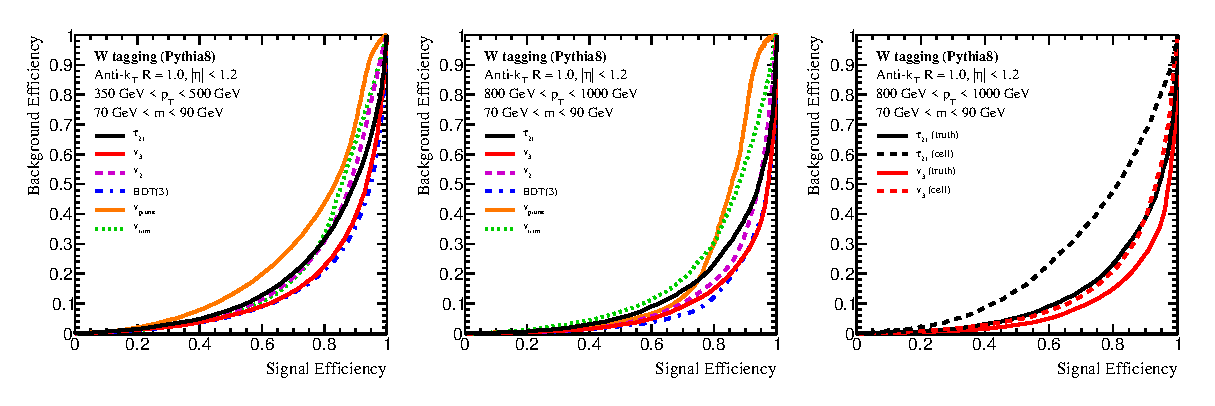
\includegraphics[width=2\columnwidth]{plots/W_ROCs_5.eps}
    \caption{The $W$ tagging ROC curves of the variabilities $v_2$, $v_3$, $v_{\rm trim}$, and $v_{\rm prun}$,
    the BDT combinations of three telescoping subjets variables $\{v_2, v_3, \theta_2\}$, and the two-prong tagger $\tau_{21}=\tau_{2}/\tau_{1}$, in the $(300~{\rm GeV}, 500~{\rm GeV})$ jet $p_T$ bin (left panel) and the $(800~{\rm GeV}, 1~{\rm TeV})$ bin (middle panel). Right panel: ROC curves of $v_3$ and $\tau_{21}$ in the $(800~{\rm GeV}, 1~{\rm TeV})$ jet $p_T$ bin. Solid curves correspond to the ones with the truth particle information, and the dashed curves are the ones using the pseudo-calorimeter cell particle information.}
\label{ROC_W}
\end{figure*}

The study is performed using samples generated from the Monte Carlo simulations of proton-proton collisions at 13 TeV using \textsc{Pythia} 8 \cite{Sjostrand:2007gs}. Particles are clustered into jets with \textsc{FastJet} 3~\cite{Cacciari:2011ma} using the anti-$k_T$ algorithm \cite{Cacciari:2008gp} with $R=1.0$ and pseudo-rapidity $|\eta|<1.2$. We consider two jet $p_T$ regions between 350 GeV and 500 GeV as well as 800 GeV and 1 TeV to examine the transition to the highly boosted regime. The $W$ and top jets are generated by decays of the Kaluza-Klein graviton with the invariant mass at 1 or 2 TeV for the two $p_T$ bins in $gg\rightarrow G^*\rightarrow W^+W^-~{\rm or}~t\bar t\rightarrow {\rm hadrons}$. The natural width of the graviton is set to 25 GeV. The background jets are QCD dijets. To study the impact of finite detector resolution, we compare the results with the particles clustered in pseudo-calorimeter $(\eta,\phi)$ cells of size $0.1\times 0.1$, with each cell momentum constructed with zero mass and direction from the primary vertex. Also, in reality pileup contamination can be an issue, especially in high-luminosity LHC runs. For this reason, we groom all the jets using jet trimming with $R_{\rm sub}=0.3$ and $f_{\rm cut}=0.05$ before the analysis except in telescoping jet grooming. We impose a trimmed jet mass cut between 70 GeV and 90 GeV for $W$ tagging and between 160 GeV and 190 GeV for top tagging.

\begin{figure*}
    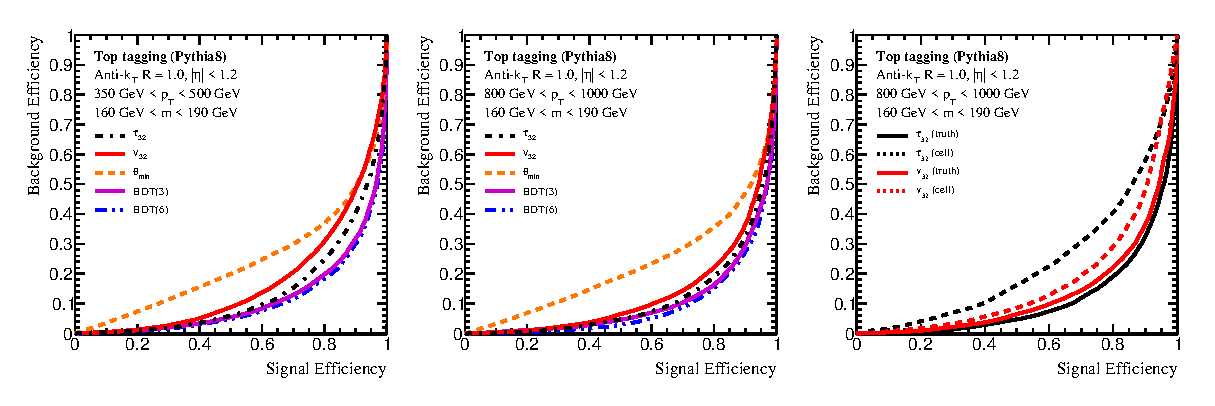
\includegraphics[width=2\columnwidth]{plots/Top_ROCs_1.eps}
    \caption{The top tagging ROC curves of the variability ratio $v_{32}$, the minimal angle among three subjets $\theta_{\rm min}$, the BDT combinations of three and six telescoping subjets variables $\{m_{W2},v_2,v_3\}$ and $\{\theta_2,\theta_{\rm min},m_{W2},v_2,v_3,v_{m_{W2}}\}$, and the three-prong tagger $\tau_{32}=\tau_{3}/\tau_{2}$, in the $(300~{\rm GeV}, 500~{\rm GeV})$ jet $p_T$ bin (left panel) and the $(800~{\rm GeV}, 1~{\rm TeV})$ bin (middle panel). Right panel: ROC curves of $v_{32}$ and $\tau_{32}$ in the $(800~{\rm GeV}, 1~{\rm TeV})$ jet $p_T$ bin. Solid curves correspond to the ones with the truth particle information, and the dashed curves are the ones using the pseudo-calorimeter cell particle information.}
\label{ROC_top}
\end{figure*}

To examine the information contained in the telescoping subjets variables, subsets of them are inputs for Boosted Decision Trees (BDTs) implemented in \textsc{TMVA} \cite{Hocker:2007ht}. %Exploiting the full information contained in the subjet variables aided with deep machine learning techniques is explored in \cite{Chien:2017decon}.
For top tagging we also consider the ratio $v_{32}$ between $v_2$ and $v_3$,
\be
    v_{32}=\frac{v_3}{v_2}\;.
\ee
FIG. \ref{v32} shows the distributions of $v_2$, $v_3$, and $v_{32}$ for top and QCD jets. We find that top jets have a broader $v_2$ distribution and a narrower $v_3$ distribution. The large variation of the jet mass when telescoping around the two subjet axes is caused by the transition of the $W$ from being partially reconstructed to fully reconstructed. There is not an intrinsic mass scale dictating the third hard emission for QCD jets. On the other hand, the three prongs inside top jets are quark-initiated subjets, whereas the subjets in QCD jets can have gluonic origins. Quark subjets are narrower than gluon subjets; therefore $v_3$ of top jets is statistically smaller. $v_{32}$ has almost the same performance as the BDT with input $\{v_2,v_3\}$, suggesting that $v_{32}$ may be the optimal way of combining the two variabilities.

An interesting feature of $v_{32}$ is that it cuts off naturally and sharply at 1, most clearly seen in QCD jets. Crucially, $v_{3} \leq v_{2}$. The two-prong structure in QCD jets implies that $v_{2}$ and $v_{3}$ collect almost the same information. The third energy flow axis can not be displaced far from the two axes determined at $N=2$. Hence, little new information is collected by constructing a third subjet and the distribution of $v_{32}$ for QCD jets peaks at 1. In the case where there is a third, semi-hard emission, $v_{3} < v_{2}$ since the emission is captured by all telescoping subjets at $N=3$ and does not induce the observable variation. In general, since more particles are by-default captured at larger $N$, the variability decreases: $v_{N+1}\leq v_{N}$.

The performances of the observables can be illustrated by receiver operating characteristic (ROC) curves, plotting the background efficiency as a function of the signal efficiency, where a lower curve indicates a better tagging performance. FIG. \ref{ROC_W} shows the ROC curves of $v_2$, $v_3$, $v_{\rm trim}$, $v_{\rm prun}$, the BDT combinations of the telescoping subjets variables $\{v_2, v_3, \theta_2\}$, and the two-prong tagger $\tau_{21}=\tau_{2}/\tau_{1}$ in $W$ tagging. The left and middle panels correspond respectively to two jet $p_T$ regions of $(350~{\rm GeV}, 500~{\rm GeV})$ and $(800~{\rm GeV}, 1~{\rm TeV})$. Overall the tagging performance increases at higher $p_T$ which shows the general advantage of applying telescoping to the boosted regime. We find the excellent performance of $v_3$ and its qualitatively different feature compared to $\tau_{21}$. In the right panel we compare the tagging performances using truth particle information and pseudo-calorimeter clusters, which destroy information about structures smaller than their cell size. We find that $v_3$ is much more robust against the smearing, especially at high $p_T$. $v_3$ utilizes the $W$ isolation and probes the rapid depletion of radiation around the $W$ at larger angles in the boosted regime. This is the manifestation of the fact that the $W$ carries zero color charge which affects the color structure of the subjets. The time dilation that occurs before $W$ hadronically decays can also create a huge difference from QCD jets in the jet formation process. On the other hand, the fact that $v_3$ performs better than $v_2$ hints at the significance of a third hard emission in $W$ and QCD jets, and $v_3$ disentangles that effect in the quantification of the $W$ isolation. The physics picture of $v_{\rm trim}$ and $v_{\rm prun}$ is still under study.

FIG. \ref{ROC_top} shows the ROC curves for top tagging: $v_{32}$, $\theta_{\rm min}$, the BDT combinations of telescoping subjets variables $\{v_2, v_3, m_{W2}\}$ and $\{\theta_2,\theta_{\rm min},m_{W2},v_2,v_3,v_{m_{W2}}\}$, and the three-prong tagger $\tau_{32}=\tau_{3}/\tau_{2}$. Again the left and middle panels correspond to the $(350~{\rm GeV}, 500~{\rm GeV})$ and $(800~{\rm GeV}, 1~{\rm TeV})$ jet $p_T$ regions respectively, and we note tagging performance increases at higher $p_T$. In the right panel the ROC curves plot both truth-particle and pseudo-calorimeter information. We find the excellent performance of $v_{32}$ and its robustness against smearing, especially at high $p_T$ where the performance of $\tau_{32}$ degrades dramatically. This indicates the qualitatively different features of $v_{32}$ and a three-prong tagger. We also find the usefulness of including $m_{W2}$ in the minimal BDT combination which significantly increases the tagging performance. It is clear that the intrinsic mass scale $M_W$ within the top jet is a unique feature distinguishing itself from the QCD background. One may also start to see the $W$ isolation within the top jet in the boosted regime.

To conclude, we introduce a %differential
jet substructure calculus using variability to quantify the change of observables with respect to the variation of the phase-space boundary in the observable definition. The method is general and can be used to analyze arbitrary classes of jet substructure observables and grooming procedures. We apply telescoping jet substructure in $W$ and top tagging and focus on telescoping subjets. We find the excellent performances of $v_3$ in $W$ tagging and $v_{32}$ in top tagging. Their robustness is demonstrated by comparing the performances using the truth particles and the %calorimeter-smeared
pseudo-calorimeter information. On the other hand, we find that the performance of typical $N$-prong taggers, like $\tau_{21}$ in $W$ tagging and $\tau_{32}$ in top tagging. decreases dramatically in the boosted regime in calorimeter settings. This shows that the variability is a qualitatively new feature of jets. We also find the usefulness of exploiting the intrinsic $W$ mass scale within the top jet by the significant increase of the tagging performance in the BDT combination.

The new physics messages we learn include the emergence of the isolation of $W$ jets at high $p_T$, which is a dominant feature over their two-prong structure. This is true for all other heavy, color-singlet Standard Model particles including the $Z$ and the Higgs boson. The top jet also has features beyond the three-prong structure which can be exploited to increase tagging performance. The telescoping subjets provides a systematic framework within which one can construct qualitatively new jet substructure observables. This paves the road toward complete and systematic jet studies using telescoping deconstruction \cite{Chien:2017decon}.




\section{Acknowledgements}
Y.-T. Chien would like to thank the organizers of the BOOST2015 conference where telescoping jet substructure was first presented. Y.-T. Chien was supported by the US Department of Energy (DOE), Office of Science under Contract No. DE-AC52-06NA25396, the DOE Early Career Program and the LHC Theory Initiative Postdoctoral Fellowship under the National Science Foundation grant PHY-1419008. A. Emerman was supported by the National Science Foundation under Grant No. PHY-1707971. S.-C. Hsu and S. Meehan were supported by the DOE Office of Science, Office of High Energy Physics Early Career Research program under Award Number DE-SC0015971. Z. Montague was supported by the University of Washington's Ernest M. Henley \text{\&} Elaine D. Henley Endowed Fellowship.


\bibliography{TJet_ref}
\end{document}






















